\documentclass{article}
\usepackage{amsmath, amssymb, amsfonts, amsthm}
\usepackage[margin=1in]{geometry}
\usepackage{fancyhdr}
\usepackage[final]{pdfpages}
\usepackage[makeroom]{cancel}
\usepackage{enumitem}

\usepackage[normalem]{ulem} 

\newcommand{\lecture}[3]{
   \pagestyle{myheadings}
   \thispagestyle{plain}
   \newpage
   \setcounter{page}{1}
   \noindent
   \begin{center}
   \framebox{
      \vbox{\vspace{2mm}
      \hbox to 6.28in { {\bf CSCI-4968: ML and Optimization}
      \hfill Spring 2023 }
        \vspace{5mm}
        \hbox to 6.28in { {\Large \hfill #1 \hfill} }
        \vspace{2mm}
         \hbox to 6.28in { {\it #2 \hfill #3 \ \ \ } }
        % \vspace{2mm}
      }
   }
   \end{center}
   \markboth{Lecture: #1: #2}{Lecture: #1: #2}
}

\begin{document}

\lecture{Semidefinite Programming}{}{For approximating Max Cut and Travelling Salesman}

\section{Motivation}
\textbf{\textcolor{red}{TODO: Update this section (matrix completion)}}
\subsection{Max Cut} % algorithm listings
\textbf{\textcolor{red}{TODO: Fix}}
We would like to partition our graph into two set of vertices such that the sum of the edge weights between the two partitiions is maximized. 

Applications include 
examples: Clustering
- Intuition: The distances between the two partitiions are the greatest so they have a high likelihood of belonging to two different categories. 

\subsection{Travelling Salesman Problem} % algorithm listings
\textbf{\textcolor{red}{TODO: Fix}}
Imagine you are prospective student touring RPI. You have a list of buildings you want to visit.
You have on hand the distance between each pair of buildings. 
Is it possible to find a path such that each buidling is visited exactly once? 
If so, what is the shortest possible distance you will need to travel. 
Since you toruing the college, it is likely you have some method of transportation to came from and need to come back to . 
We have the added constraint that you start at the parking lot and will need to come back to the parking lot.
This is know as the travelling salesman.
% One sentence Goal
As our goal is to find an \emph{efficient} route, we will be satisfied with an approximation. 
Or a series of buidlings to visit that is close the optimal.


% How is this different form the max cut 

\section{Semidefinite Programming}  % objective functions

\subsection{Recap of Linear Programming}
To give background on semi-definite programming, we begin with a brief recap of linear programming.
Suppose that you have control over a set of variables and you are attempting to find a selection for each of these variables such that some linear combination is either maximized or minimized.
To give background on semi-definite programming we first start with a brief recap of linear programming.
To make this more complicated suppose that these variables each have a constraint that must be met.

Formally we can write this out as the following. Suppose that we have \( n \) variables that we have control over which we can represent as:
\[
\vec{x} = \begin{bmatrix} x_1 \\ x_2 \\ \vdots \\ x_n \end{bmatrix}
\]

This problem is made trivial by setting \( \vec{x} \) to be arbitrarily large or small value depending on the optimization direction.
The solution becomes more meaningful if the domain of each variable is constrainted.

Say for each of these \( n \) variables has an associated coefficient \( \vec{c} = \begin{bmatrix} c_1, c_2, ..., c_n  \end{bmatrix}^\top \).
We would like to find \( \vec{x} \) such that the linear combinatrion of the two (\( \vec{c} \cdot \vec{x} \)) is minimized
\begin{align*}
  \begin{array}{ll@{}ll}
  \min  & \vec{c} \cdot \vec{x}
  \end{array}
\end{align*}

We can extend this idea to a system of equations. We define \( \vec{a}_i \) and \( \vec{b} \) to vectors in $\mathbb{R}^n$. We would like to find \( \vec{x} \) such that
\begin{align*}
\vec{a}_1 \cdot \vec{x} &= b_1 \\
\vec{a}_2 \cdot \vec{x} &= b_2 \\
& \vdots  \\
\vec{a}_n \cdot \vec{x} &= b_n \\
\end{align*}

Graphically, each constraint creates a \emph{half-space}. 
The intersection of the halfspaces (the white space) is our solution set. 
Our goal is the find the minimize value of the intersections.
\begin{center}
  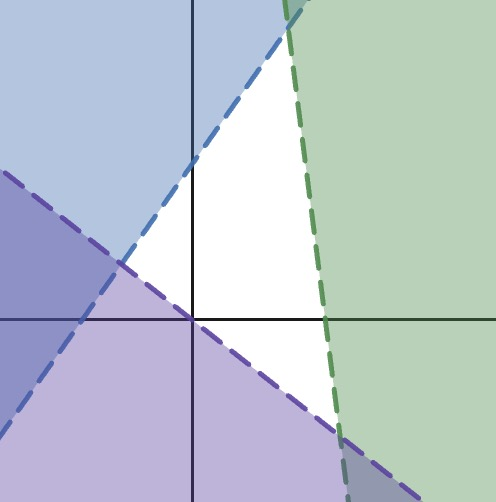
\includegraphics[scale=.2]{assets/half_space.jpg}  
\end{center}

We can gather our \( \vec{a}_i \) vectors into a single matrix. 
Let $\mathbf{A} = [\vec{a_1}^\top \cdots \vec{a_n}^\top]$.
so that we only need to solve:
\[
\mathbf{A} \vec{x} = \vec{b}
\]

In summary, a linear programming asks for an optimal solution, \( \vec{x} \), given a set of linear constraints
\begin{align*}
  \begin{array}{ll@{}ll}
    \text{minimize} & \vec{c} \cdot \vec{x}&\\
    \text{subject to}& \mathbf{A} \vec{x} = \vec{b} \\
    & \vec{x} \geq 0 \\
    \end{array}
\end{align*}

It is needed that \( \vec{x} \) is nonnegative (\( \vec{x} \geq 0 \)). We note that our constraints form a convex set.
Thus, linear programming is a subset of a convex optimization problem.
Finding a solution to an instance of linear programming can be done with a variety of algorithms including the \emph{simplex algorithm}.

Many real world problems can be modelled as a set of linear contraints. One use case arises in manufacturing.
Given a set of products, how much of each kind should be produced to either minimize cost or maximize profits?
Linear programming is a general approach of taking a constrained linear optimization problem into a form where a solution can easily be found.
% linear programming usable in a large variety of problems such as

\subsection{Formalization of Semidefinite Programming}
Instead of having just \( n \) variables that we have a matrix \( \mathbf{X} \) of \( n^2 \) elements. Thus instead of finding an optimal \( \vec{x} \) we are trying to find an optimal \( \mathbf{X} \in \mathbb{R}^{n \times n} \) that is symmetric positive semidefinite (SPSD) such that
\begin{gather*}
\min = \sum_{i = 1}^n \sum_{j = 1}^n x_{i, j} c_{i , j} \\
\mathbf{X} \succeq 0 \\
\end{gather*}
Where \( c_{i, j} \) is the coefficient corresponding to the \( x_{i, j} \) variable and \( \mathbf{X} \succeq 0 \) ensures that \( \mathbf{X} \) is SPSD. We can gather all \( n^2 \) coefficients into a matrix \( \mathbf{C} \) and then rewrite our minimization term as:
\[
\min \mathbf{C} \bullet \mathbf{X}
\]
Where the \( \bullet \) operator is simply taking the sum of all elements after doing element wise multiplication on two matricies \( \mathbf{C} \) and \( \mathbf{X} \) with the same shape. Formally we can write it as:
\[
  \mathbf{C} \bullet \mathbf{X} = \sum_{i = 1}^n \sum_{j = 1}^n \mathbf{C}_{i, j} \mathbf{X}_{i, j}
\]
Of important note is the fact that \( \mathbf{C} \bullet \mathbf{X} = \text{trace}(\mathbf{C}^\top \mathbf{X}) \) where \( \text{trace} \) is the sum of the diagonal terms for a matrix. Calculating the \( \text{trace} \) of the matrix multiplication is not as efficient as the \( \bullet \) operator but the notation comes up quite frequently within the literature so it is important to know.

Returning back to our formalization of SDP, we note that with more variables comes with more constraints. Suppose that we have \( n \) equations to satisfy. For each equation we have a matrix \( \mathbf{A}_i \) and a scalar value \( b_i \) defining our constraint. Then for a given constraint we have:
\[
\mathbf{A}_i \bullet \mathbf{X} = b_i
\]
This is all that is needed for SDP. We can write this out formally as:
\begin{align*}
  \min \mathbf{C} \bullet \mathbf{X} \\
  \mathbf{A}_i \bullet \mathbf{X} &= b_i  \text{   for } i = 1, 2, ..., n\\
  \mathbf{X} \succeq 0 \\
\end{align*}

The parallels between semidefinite programming and linear programming should be quite obvious.
In many ways, semidefinite programming is linear programming with more variables of control and more constraints.


\section{Relaxation}   % objective functions
\subsection{Proofs}
- performance guarantees
- proof of relaxations (how accurate + how it works)


Integrality Gap: ratio btwen optimal / relaxation 



\section{Experimental Results}
\subsection{Visualization}
- table of result
- for small examples, we find the acutal solution (brute force), or a solution (integer programming) and check how 
good our bound is

vhttps://www.cs.cmu.edu/~anupamg/adv-approx/lecture14.pdf used "randomized rounding" to find a max cut.
i.e. if $p_{ij}$ is close to -1, then we should cut it. We attempt do do something similar

\section{Discussion}


- can we prove the runtime
- can we prove how good of a lower bound we have?
- what are some easy things to prove?

\subsection{Scope and limitations}

\section{Appendix}
\newpage
\subsection{Problem Set} 

\newpage
\subsection{References}
https://www.uit.edu.mm/storage/2020/09/WWM-2.pdf

\end{document}
